%
% latex template for SRS documentation 
% name: srs.tex 
% date last modified: 22 feb 2018
% modified by: jerry 
% 
%
\documentclass{article}

\usepackage{caption}
\usepackage[margin=1in]{geometry}
\usepackage{graphicx}
\usepackage{hyperref}
\usepackage{float}
\usepackage{tabularx}
\usepackage{titling}

\begin{document}

\title{
    CSC431 \\
    \vspace{0.2in}
    \textbf{Download of Public-facing Data} \\
    \large Software Requirements Specification \\
    Team \#3 
}

\author{
    Jerry Bonnell
    \and Gururaj Shriram 
    \and Erica Chang
    \and Heyu Yao
    \and Lixiong Liang
}

\date{}
\maketitle

\clearpage
\section*{Version History}

\begin{tabularx}{\textwidth}{| l | l | X | X |}
    \hline
    \textbf{Version} & \textbf{Date} & \textbf{Author(s)} & \textbf{Change Comments} \\
    \hline
         1   & \today   &    xxx       &      xxx   \\
    \hline 
            &      &           &                 \\
    \hline
            &      &           &                 \\
    \hline             
\end{tabularx}

\clearpage
	\tableofcontents

\clearpage
	\listoffigures
	\listoftables

\clearpage

\section{System Requirements}

\subsection{Functional Requirements}

\subsubsection{Requirement Title}

\begin{table}[H]
\caption{Table title}
\begin{tabularx}{\textwidth}{|l|X|}
    \hline
    \textbf{Title} & Insert title \\ \hline
    \textbf{Description} &  A one or two sentence description \\ \hline 
    \textbf{Source Scenario} &  Code for associated scenario in SCD \\ \hline
    \textbf{Priority} &  Priority from 0 (highest) - 5 (lowest) \\ \hline 
    \textbf{Precondition(s)} &  What needs to happen before \\ \hline
    \textbf{Postcondition(s)} &  What happens as a result \\ \hline
    \textbf{Use Case Diagram} &  Link or number, if present \\  \hline                 
\end{tabularx}
\end{table}

\subsection{Non-Functional Requirements}


\subsubsection{Requirement Title}

\begin{table}[H]
\caption{Table title}
\begin{tabularx}{\textwidth}{|l|X|}
    \hline
    \textbf{Title} & Insert title \\ \hline
    \textbf{Description} &  A one or two sentence description \\ \hline 
    \textbf{Source Scenario} &  Code for associated scenario in SCD \\ \hline
    \textbf{Priority} &  Priority from 0 (highest) - 5 (lowest) \\ \hline 
    \textbf{Applicable FR(s)} &  What functional requirement(s) is this applicable to? \\ \hline            
\end{tabularx}
\end{table}

\pagebreak

\section{System Constraints}

\subsection{Tool Constraints}

\subsubsection{Requirement Title}

\begin{table}[H]
\caption{Table title}
\begin{tabularx}{\textwidth}{|l|X|}
    \hline
    \textbf{Title} & Insert title \\ \hline
    \textbf{Description} &  A one or two sentence description \\ \hline 
    \textbf{Priority} &  Priority from 0 (highest) - 5 (lowest) \\ \hline       
\end{tabularx}
\end{table}

\subsection{Language Constraints}

\subsubsection{Requirement Title}

\begin{table}[H]
\caption{Table title}
\begin{tabularx}{\textwidth}{|l|X|}
    \hline
    \textbf{Title} & Insert title \\ \hline
    \textbf{Description} &  A one or two sentence description \\ \hline 
    \textbf{Priority} &  Priority from 0 (highest) - 5 (lowest) \\ \hline       
\end{tabularx}
\end{table}

\subsection{Platform Constraints}

\subsubsection{Requirement Title}

\begin{table}[H]
\caption{Table title}
\begin{tabularx}{\textwidth}{|l|X|}
    \hline
    \textbf{Title} & Insert title \\ \hline
    \textbf{Description} &  A one or two sentence description \\ \hline 
    \textbf{Priority} &  Priority from 0 (highest) - 5 (lowest) \\ \hline       
\end{tabularx}
\end{table}

\subsection{Hardware Constraints}

\subsubsection{Requirement Title}

\begin{table}[H]
\caption{Table title}
\begin{tabularx}{\textwidth}{|l|X|}
    \hline
    \textbf{Title} & Insert title \\ \hline
    \textbf{Description} &  A one or two sentence description \\ \hline 
    \textbf{Priority} &  Priority from 0 (highest) - 5 (lowest) \\ \hline       
\end{tabularx}
\end{table}

\subsection{Network Constraints}

\subsubsection{Requirement Title}

\begin{table}[H]
\caption{Table title}
\begin{tabularx}{\textwidth}{|l|X|}
    \hline
    \textbf{Title} & Insert title \\ \hline
    \textbf{Description} &  A one or two sentence description \\ \hline 
    \textbf{Priority} &  Priority from 0 (highest) - 5 (lowest) \\ \hline       
\end{tabularx}
\end{table}

\subsection{Deployment Constraints}

\subsubsection{Requirement Title}

\begin{table}[H]
\caption{Table title}
\begin{tabularx}{\textwidth}{|l|X|}
    \hline
    \textbf{Title} & Insert title \\ \hline
    \textbf{Description} &  A one or two sentence description \\ \hline 
    \textbf{Priority} &  Priority from 0 (highest) - 5 (lowest) \\ \hline       
\end{tabularx}
\end{table}

\subsection{Transition \& Support Constraints}

\subsubsection{Requirement Title}

\begin{table}[H]
\caption{Table title}
\begin{tabularx}{\textwidth}{|l|X|}
    \hline
    \textbf{Title} & Insert title \\ \hline
    \textbf{Description} &  A one or two sentence description \\ \hline 
    \textbf{Priority} &  Priority from 0 (highest) - 5 (lowest) \\ \hline       
\end{tabularx}
\end{table}

\subsection{Budget \& Schedule Constraints}

\subsubsection{Requirement Title}

\begin{table}[H]
\caption{Table title}
\begin{tabularx}{\textwidth}{|l|X|}
    \hline
    \textbf{Title} & Insert title \\ \hline
    \textbf{Description} &  A one or two sentence description \\ \hline 
    \textbf{Priority} &  Priority from 0 (highest) - 5 (lowest) \\ \hline       
\end{tabularx}
\end{table}

\subsection{Miscellaneous Constraints}

\subsubsection{Requirement Title}

\begin{table}[H]
\caption{Table title}
\begin{tabularx}{\textwidth}{|l|X|}
    \hline
    \textbf{Title} & Insert title \\ \hline
    \textbf{Description} &  A one or two sentence description \\ \hline 
    \textbf{Priority} &  Priority from 0 (highest) - 5 (lowest) \\ \hline       
\end{tabularx}
\end{table}

\clearpage

\section{Requirements Modeling}

\subsection{Requirement Title}

\begin{figure}[H]
  \begin{center}
    \caption{Sample Use Case}
    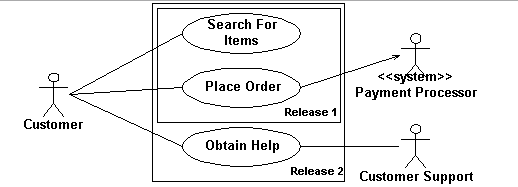
\includegraphics{images/sample_use_case.png}
  \end{center}
\end{figure}

\clearpage

\section{Evolutionary Requirements}

\subsection{Functional Requirements}

\subsubsection{Requirement Title}

\begin{table}[H]
\caption{Table title}
\begin{tabularx}{\textwidth}{|l|X|}
    \hline
    \textbf{Title} & Insert title \\ \hline
    \textbf{Description} &  A one or two sentence description \\ \hline 
    \textbf{Priority} &  Priority from 0 (highest) - 5 (lowest) \\ \hline 
    \textbf{Precondition(s)} &  What needs to happen before \\ \hline
    \textbf{Postcondition(s)} &  What happens as a result \\ \hline
    \textbf{Use Case Diagram} &  Link or number, if present \\  \hline                 
\end{tabularx}
\end{table}

\subsection{Functional Requirements}

\subsubsection{Requirement Title}

\begin{table}[H]
\caption{Table title}
\begin{tabularx}{\textwidth}{|l|X|}
    \hline
    \textbf{Title} & Insert title \\ \hline
    \textbf{Description} &  A one or two sentence description \\ \hline 
    \textbf{Priority} &  Priority from 0 (highest) - 5 (lowest) \\ \hline 
    \textbf{Applicable FR(s)} &  What functional requirement(s) is this applicable to? \\ \hline            
\end{tabularx}
\end{table}


\end{document}